\section{Vulkan}
Vulkan is a new generation graphics and compute API that provides high-efficiency, cross-platform access to modern GPUs used in a wide variety of devices from PCs and consoles to mobile phones and embedded platforms \cite{vulkan}.

\subsection{Validation layers}
The Vulkan API is designed around the idea of minimal driver overhead and one of the manifestations of that goal is that there is very limited error checking in the API by default. Even mistakes as simple as setting enumerations to incorrect values or passing null pointers to required parameters are generally not explicitly handled and will simply result in crashes or undefined behavior \cite{vulkan_tutorial}. Vulkan comes with a set of validation and debug layers as part of the Vulkan SDK. When any subset of these layers are enabled they insert themselves automatically into the call-chain of every Vulkan API call issued by the application to perform their job. Validation layers can also report warnings about potential incorrect or dangerous use of the API, and are even capable of reporting performance warnings that allow developers to identify places where the API is used correctly but not used in the most efficient way \cite{vulkan_validation_layers}.

\subsection{Memory management}
While OpenGL drivers manage memory allocations transparently to the programmer, Vulkan not only allows but also requires that programmers allocate device memory (in our case, GPU memory) and bind the memory to the resources used in the application. While this may increase the application's performance if the programmer takes advantage of it, it also requires the programmer to manually manage buffer alignments and aliasing.  The recommended way of allocating memory and creating buffers is described in Figure \ref{fig:vulkan_mem_alloc}.

\begin{figure}[ht]
    \centering
    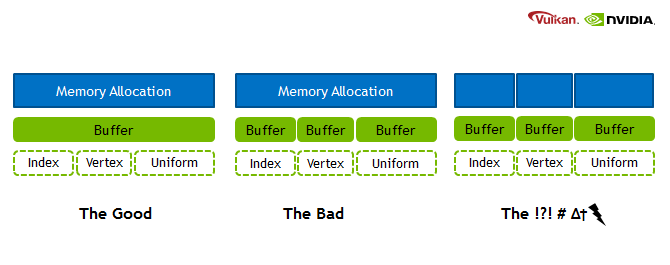
\includegraphics[width = 15cm]{figs/vulkan_memory_strategy.png}
    \caption{Vulkan memory allocation strategies}
    \label{fig:vulkan_mem_alloc}
\end{figure}

The diagram in figure \ref{fig:vulkan_mem_alloc} illustrates three memory allocation strategies \cite{vulkan_mem_mgmt}.
The rightmost is the naive approach: for each buffer is performed a "dedicated" memory allocation. This approach is the easiest to implement, since every object allocates, binds and frees their own memory, without taking into account other objects created. It is also the least optimized approach, given that this most likely will not be cache-friendly. It is also important to note that Vulkan devices have a maximum number of memory allocations that can exist simultaneously;
The approach shown in the middle, captioned "The Bad", shows a single memory allocation with various buffers bound to it. This approach is more cache-friendly than the previous one, but it requires the programmer to deal with memory aliasing, offsets and buffer alignments;
The leftmost, captioned as "The Good", is the recommended approach. It represents a single memory allocation bound to a single buffer, with different data loaded to different areas of the buffer. This approach is the most cache-friendly and the most optimized for performance in highly dynamic scenes, but also the most difficult to implement. This setup is possible thanks to Vulkan low-level control of offsets even inside a single buffer, allowing the developer to define "virtual buffers".

In this work, our goal was to allow the user to build simple scenes with few objects, for the purposes of visualization only. For this reason, we opted to use the naive approach. Implementing a memory management module would not perceivably impact on the performance of the application.

\subsection{Compiling shaders}
Up until OpenGL 4.6, application had to be compile shader source code at run-time, passing a string of high-level source code to the graphics driver. While this allowed the application to run on different hardware, this also forced each GPU manufacturer to provide a GLSL compiler with the device driver, making it difficult for vendors to update and support new versions of the API in their drivers.

\subsubsection{SPIR-V}
The "Standard Portable Intermediate Representation" version "V" (as in "Vulkan") is a binary representation of shader code which device drivers can parse more easily. Application developers, having their shaders written, must compile them into SPIR-V format before loading them in their applications. This contributes for quicker development of device drivers. Support for SPIR-V shaders is included in OpenGL 4.6 and Vulkan 1.0.
